\section{Implementation}
In this section, we show how we applied the general idea for multilingual
program analysis into implementing the dataflow analysis tool for JNI programs
using CodeQL, which we named JN-QL. CodeQL is a static analysis engine that
transforms source code into database, and performs analysis by evaluating
"query", written in declarative language called QL (Query langague). In QL,
defining data-facts and rules are referred as defining "predicates", which has
the following form:
\begin{lstlisting}[style=codeql,xleftmargin=2.5em]
predicate isOneTwoThree(int n) {
  n = 1
  or
  n = 2
  or
  n = 3
}
\end{lstlisting}

QL is also object-oriented language, so that it support class definition:
\begin{lstlisting}[style=codeql,xleftmargin=2.5em]
class OneTwoThree extends int {
  OneTwoThree() { // characteristic predicate
    this = 1
    or
    this = 2
    or
    this = 3
  }
}
\end{lstlisting}

Basically, defining class is not really different to defining predicate,
as class is just set of elements that satisfy the predicate called
"characteristic prdicate". For more detailed information about QL, one
refer to the paper[6] or the official document[7].

\begin{figure}[t]
  \centering
  \vspace{2mm}
  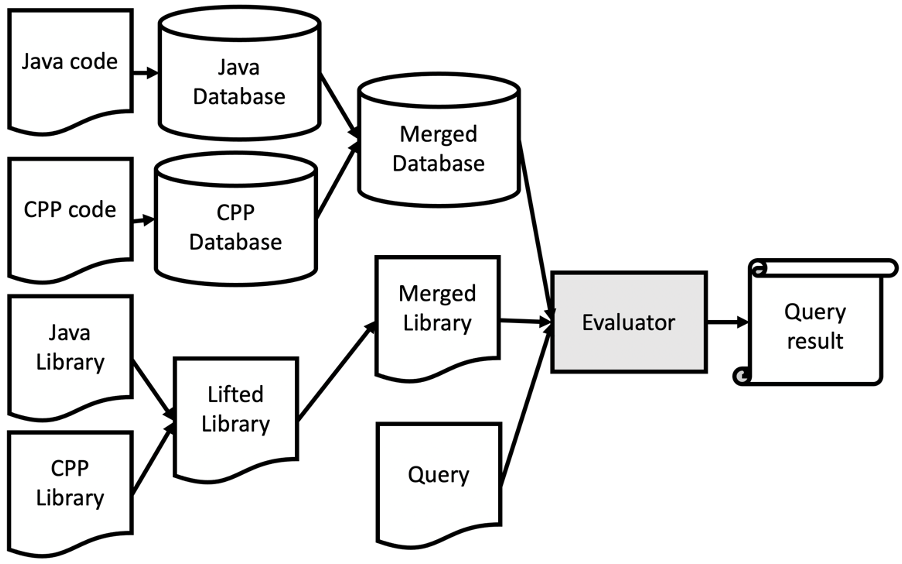
\includegraphics[width=0.5\textwidth]{img/Fig1}
  \vspace*{-1.5em}
  \caption{the overview of how declarative style analysis can be
  extended to multilingual analysis}
  \label{fig:Fig1}
\vspace*{-.5em}
\end{figure}

Figure~\ref{fig:Fig1} shows the overall structure of JN-QL. First, it generates database
for each language, C++ and Java, and merge it to one database. This corresponds to a step of
extracting syntactic data-facts from the source code. Then, we merge two
existing dataflow analysis framework, which are part of the library that 
CodeQL provides as a form of library, into one merged library. Finally, using the
merged database and merged library, the user can write a query to perform the
client-analysis, and evaluate it to get analysis result.

\subsection{Create database}
The first step is to gernerate database for each of two languages.  For
compiled languages such as C++ and Java, CodeQL generates database by running
the compiler for each language. While the compiler is running, CodeQL monitors
the behavior of compiler and extracts information it needs, and create database
with that information.  Creation of database for one language is performed in
two steps: first, the extracted information from compiler is stored in the
human readable file format called trap files, and second, these trap files are
then finalized into database, written in binary format.

[Insert example of trap file here]

In order to create a database for two languages, JN-QL performs first step for
each languages separately to get two sets of trap files.  Next step would be to
perfrom finalization step on merged set of trap files. However, a problem is that
both of trap files have table with duplicated name, so simply mering them would not work.
The solution is to add prefix to name of each table. For example, if both
database have tables named "@expr", the table from C++ would be renamed as
"@cpp\_expr", and the table from Java would be renamed as "@java\_expr". After
renaming each table, the second step can be applied to finalize the database on
which the query can be evaluated.

\subsection{Lift library}
CodeQL provides various libraries for each languages, which consists of some
pre-defined predicates and classes that can be useful for user to implement
analysis on their own taste. Dataflow analysis library is one of them, and both
C++ and Java supports this dataflow anslysis library. Two dataflow analysis
library have same framework: they share same classes such as "Node", and some
predicates such as "simpleLocalFlowStep".

\begin{lstlisting}[style=codeql,xleftmargin=2.5em]
class Node extends TNode {
  ...
}
predicate simpleLocalFlowStep(Node nodeFrom, Node nodeTo) {
  // Expr -> Expr
  exprToExprStep_nocfg(
    nodeFrom.asExpr(),
    nodeTo.asExpr()
  )
  or
  // Assignment -> LValue post-update node
  ...
}
//cpp/dataflow/internal/DataFlowUtil.qll
class Node extends TNode {
  ...
}
predicate simpleLocalFlowStep(Node node1, Node node2) {
  // Variable flow steps through
  // adjacent def-use and use-use pairs.
  exists(SsaExplicitUpdate upd |
    upd.getDefiningExpr().(VariableAssign).getSource()
    = node1.asExpr() or
    upd.getDefiningExpr().(AssignOp) = node1.asExpr()
  |
    node2.asExpr() = upd.getAFirstUse()
  )
  or
  // Flow through this
  ...
}
//cpp/dataflow/internal/DataFlowUtil.qll
\end{lstlisting}
However, these two implementations are not compatible, that is, although they have the same name,
we can not use "Node" class of C++ as an argument for "simpleLocalFlowStep" predicate of Java or vice versa.
Therefore, we lift each of the library into the same level so that classes and predicates become compatible.
First, we encapsulated each of original dataflow into CodeQL's module, named CPP and JAVA so that
original classes and predicated can be distinguished with lifted ones.
A class can be lifted by first defining sum type, which denotes that the lifted class would be either from C++ or
Java, and then make the lifted class be of that type. We also implemented two member predicates that can cast
the lifted class into each of corresponding class.
\begin{lstlisting}[style=codeql,xleftmargin=2.5em]
private newtype TNode =
  TJavaNode(JAVA::Node n)
  or
  TCppNode(CPP::Node n)
class Node extends TNode {
  JAVA::Node asJavaNode() {
    this = TJavaNode(result)
  }
  CPP::Node asCppNode() {
    this = TCppNode(result)
  }
  ...
}
\end{lstlisting}

A predicate can be lifted by combining two original predicates with "or" connectives.
For each original predicate, each of the arguments and return values are casted down to
correspnding language's class. After lifting, the lifted predicate shows equlivalent behavior
as the original ones if all the arguments are from the same language.
\begin{lstlisting}[style=codeql,xleftmargin=2.5em]
predicate simpleLocalFlowStep(Node node1, Node node2) {
  JAVA::simpleLocalFlowStep(
    node1.asJavaNode(), node2.asJavaNode()
  )
  or
  CPP::simpleLocalFlowStep(
    node1.asCppNode(), node2.asCppNode()
  )
}
\end{lstlisting}
\subsection{Merge library}

After the library is lifted, the last step is to extend some predicates to reflect the
semantics of interoperation between languages. For example, the predicate named "viableCallable"
is a predicate for connecting function call and target function. It gets argument of class "DataFlowCall",
and the result is of class "DataFlowCallable". After merging the libraries, this predicate would be as follow:

\begin{lstlisting}[style=codeql,xleftmargin=2.5em]
DataFlowCallable viableCallable(DataFlowCall c) {
result.asJavaDataFlowCallable()
  = JAVA::viableCallable(c.asJavaDataFlowCall()) or
result.asCppDataFlowCallable()
  = CPP::viableCallable(c.asCppDataFlowCall()) or
result.asCppDataFlowCallable()
  = viableCallableJ2C(c.asJavaDataFlowCall()) or
result.asJavaDataFlowCallable()
  = viableCallableC2J(c.asCppDataFlowCall())
}
\end{lstlisting}

The first two lines are result of lifting, and they take advantage of the
original predicates from dataflow library.  They handle the call edges from
Java to Java, and from C++ to C++.

Next two lines are the result of merging library, and they are responsible for
inter-language call edges.  The predicate "viableCallableJ2C" finds call edges
from Java to C++, and the predicate "viableCallableC2J" finds call edges from
C++ to Java. One thing to note here is that, function call from Java to C++
and function call from C++ to Java is different. Function call from Java to C++
is mostly static, that is, the target of function call can be determined in compile
time, without requiring run-time value. On the other hand, the method call from C++
to java requires runtime value. The method call from C++ to java is done by calling
interface function: callJavaMethod(name, args...). The target
method's name is passed as a string value to the argument "name",
and in order to determine correct function call target, the value stored in the argument
should be identified. In order to correctly analyze this feature, we used "inner-flow"
to determine what string values can flow into this argument.

\subsection{JNI specific details}
\inred{Write JNI-specific implementation details here: method, class as node / identify jni call / reduce time?}
